% fig7_8.tex — 7-11: 两弹簧连接物块（水平）
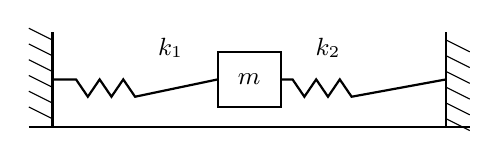
\begin{tikzpicture}[font=\small,>=stealth]
  % 左墙
  \draw[thick] (-2.5,0.6) -- (-2.5,-0.6);
  \foreach \y in {-0.5,-0.3,...,0.5}
    \draw (-2.5,\y) -- (-2.8,{\y+0.15});
  % 右墙
  \draw[thick] (2.5,0.6) -- (2.5,-0.6);
  \foreach \y in {-0.5,-0.3,...,0.5}
    \draw (2.5,\y) -- (2.8,{\y-0.15});
  % 地面
  \draw[thick] (-2.8,-0.6) -- (2.8,-0.6);
  % 左弹簧 k1
  \draw[thick] (-2.5,0) -- ++(0.3,0)
    foreach \i in {1,...,5}{
      -- ++(0.15,{(-1)^\i*0.22})
    } -- (-0.4,0);
  % 右弹簧 k2
  \draw[thick] (0.4,0) -- ++(0.15,0)
    foreach \i in {1,...,5}{
      -- ++(0.15,{(-1)^\i*0.22})
    } -- (2.5,0);
  % 物块
  \draw[thick,fill=white] (-0.4,-0.35) rectangle (0.4,0.35);
  \node at (0,0) {$m$};
  % 标注
  \node[above] at (-1.0,0.15) {$k_1$};
  \node[above] at (1.0,0.15) {$k_2$};
\end{tikzpicture}
